\section{Progettazione}
\subsection{Architettura del sistema}
Per questo progetto, essendo fondamentalmente un sistema \gls{etl}\glsadd{etl_def} ho deciso di adottare un'architettura a più livelli, che consente di separare le diverse funzionalità del sistema in moduli distinti e indipendenti.
Il primo livello è rappresentato dai servizi \textit{honeypot}, che simulano i servizi di rete vulnerabili e raccolgono i \textit{log} delle attività sospette.
Il secondo livello è costituito dai \textit{script} di raccolta e trasferimento dei \textit{log}, che elaborano i dati raccolti e li inviano al database.
Il terzo livello è rappresentato dal \textit{database} \textit{InfluxDB}, che memorizza i \textit{log} in modo strutturato e consente di eseguire query sui dati.
Infine, i dati vengono visualizzati tramite \textit{Grafana}, che offre un'interfaccia intuitiva per l'analisi e la visualizzazione delle informazioni.
\begin{figure}[H]
    \begin{center}
    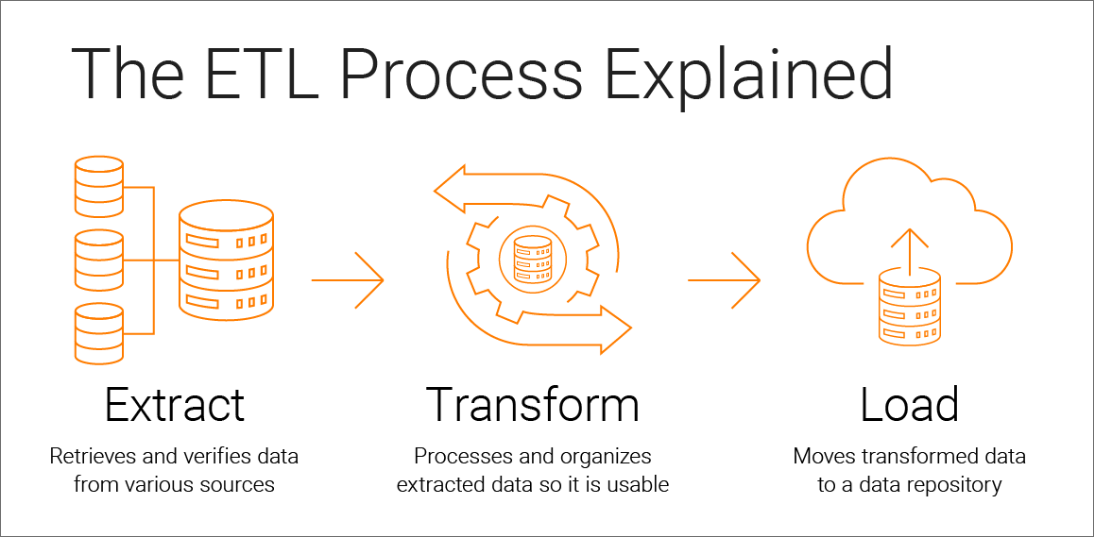
\includegraphics[width=0.9\textwidth]{img/etl-process-explained-diagram.png}
    \caption{Architettura del sistema \textit{ETL}.}
    Fonte: \url{https://www.informatica.com/resources/articles/what-is-etl.html}
    \label{fig:etl-architecture}
    \end{center}
\end{figure}
Partendo da questa architettura di base, ho progettato il sistema in maniera tale da essere modulare e scalabile, in modo da poter aggiungere facilmente nuovi servizi vulnerabili al sistema \textit{honeypot} o modificare quelli esistenti senza influire sulle altre componenti.
Ho quindi prodotto il seguente diagramma di flusso che rappresenta il funzionamento generale del prodotto, dalla raccolta dei \textit{log} alla loro visualizzazione.
\begin{figure}[H]
    \begin{center}
    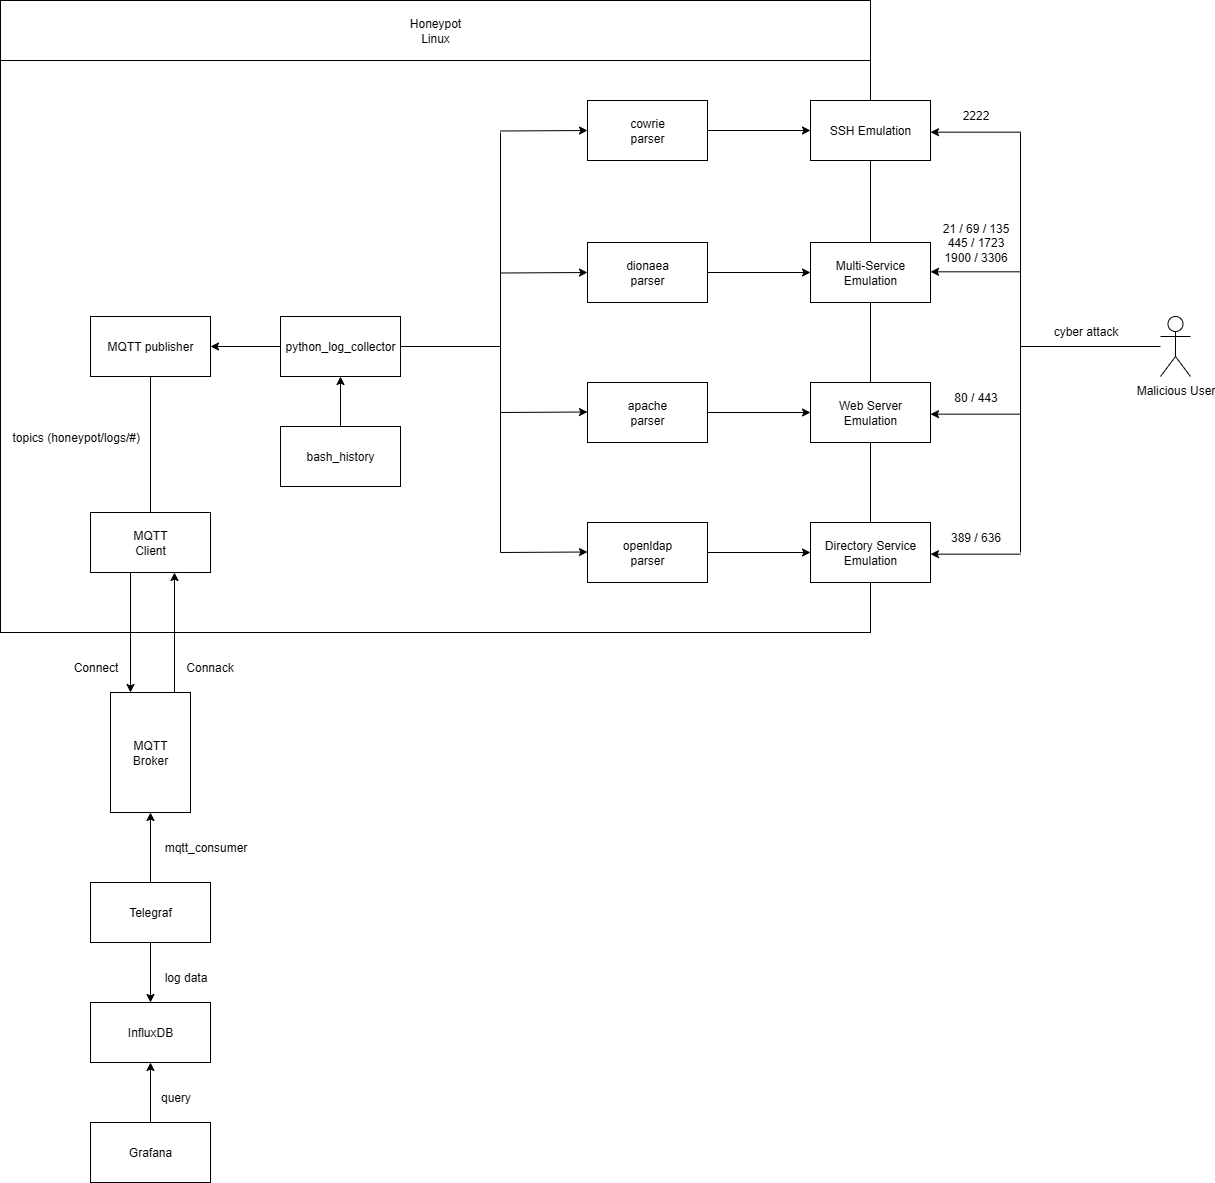
\includegraphics[width=1.025\textwidth]{img/Diagramma-flusso.png}
    \caption{Diagramma di flusso del sistema \textit{honeypot}.}
    \label{fig:flowchart}
    \end{center}
\end{figure}
Il diagramma mostra come i \textit{log} vengano generati dai servizi vulnerabili in seguito a tentativi di accesso o attacchi.
Gli \textit{script} di monitoraggio raccolgono i \textit{log}, li elaborano e li pubblicano su un \textit{topic} tramite un \textit{publisher} del protocollo \textit{MQTT}.
\textit{Telegraf}, poi, preleva i dati dal \textit{topic} e li invia al database \textit{InfluxDB} per la memorizzazione.
Infine, \textit{Grafana} consente di visualizzare i dati memorizzati nel database tramite \textit{dashboard} personalizzate.
\subsection{Scelta dei servizi del sistema}
Il sistema \textit{honeypot} doveva risultare realisticamente vulnerabile, in modo da attirare l'attenzione di potenziali attaccanti e raccogliere dati utili per l'analisi delle minacce. 
Per questo motivo abbiamo selezionato servizi noti per le loro vulnerabilità e diffusione, in grado di coprire una varietà di protocolli e tecnologie. 
La scelta è ricaduta su \textit{Cowrie}, \textit{Dionaea}, \textit{Apache} e \textit{OpenLDAP}. Ho scelto e configurato ciascuno di questi servizi per scenari d'attacco specifici e per fornire dati di valore durante il processo di monitoraggio.\\\\
\textbf{Cowrie} è un servizio progettato per emulare un sistema \textit{Linux} accessibile tramite protocollo \gls{ssh}\glsadd{ssh_def}. La sua funzione principale è quella di raccogliere informazioni su tentativi di accesso non autorizzato e sulle attività post-compromissione degli attaccanti. 
Per questo motivo l'ho configurato per ascoltare sulla porta 2222, simulando un server \textit{SSH} con un ambiente Linux realistico. 
Cowrie offre un \textit{file system} virtuale, l'emulazione di numerosi comandi \textit{bash} e il \textit{logging} completo delle sessioni, registrando anche eventuali \textit{upload} o \textit{download} di file tramite \gls{scp}\glsadd{scp_def} o \textit{wget}. 
La sua capacità di simulare vulnerabilità comuni lo rende particolarmente adatto a intercettare interazioni malevole e a raccogliere indicatori di compromissione.\\\\
\textbf{Dionaea}, invece, l'abbiamo scelto per la sua capacità di emulare più servizi vulnerabili contemporaneamente e di catturare \textit{payload} malevoli. 
Questo lo rende particolarmente utile nell'osservare attacchi automatizzati mirati a protocolli obsoleti o insicuri. 
Il \textit{container} l'ho configurato per ascoltare su diverse porte critiche: la 21 (\textit{FTP}), la 69 (\gls{tftp}), la 445 (\textit{SMB}), la 135 (\gls{rpc})\glsadd{rpc_def}, la 1723 (\gls{pptp}\glsadd{pptp_def}) e la 3306 (\textit{MySQL}). 
In questo modo \textit{Dionaea} è in grado di registrare tentativi di \textit{brute-force}, trasferimenti di file sospetti, comandi \gls{sql}\glsadd{sql_def} malevoli e attacchi legati a vulnerabilità precedentemente sfruttate. 
La sua versatilità consente di coprire un ampio spettro di minacce legate a servizi di rete differenti.\\\\
\textbf{Apache} lo abbiamo incluso per la sua enorme diffusione come server \textit{web} e per la frequente presenza di vulnerabilità legate al mondo delle applicazioni \textit{web}. 
Configurato per rispondere sulle porte 80 (\gls{http}\glsadd{http_def}) e 443 (\gls{https}\glsadd{https_def}), può essere utilizzato per simulare scenari di attacco tipici del \textit{web}, come \textit{directory traversal}, \textit{upload} di file non autorizzati, \gls{xss}\glsadd{xss_def} o altre iniezioni lato server. 
In tal modo è possibile raccogliere dati relativi a una delle superfici di attacco più comuni e sfruttate dagli attori malevoli.\\\\
Infine, l'ho integrato \textbf{OpenLDAP}, scelto per simulare un servizio di directory largamente utilizzato in ambito aziendale per l'autenticazione e la gestione centralizzata degli utenti. 
Il \textit{container} l'ho configurato per esporre sia la porta 389 (\gls{ldap} in chiaro) sia la 636 (\gls{ldaps} cifrato). 
Questa configurazione consente di osservare tentativi di enumerazione utenti, iniezione \textit{LDAP} e altre tecniche di compromissione legate a \textit{directory service}, che rappresentano spesso un obiettivo strategico per gli attaccanti al fine di ottenere accessi privilegiati.
La combinazione di questi servizi consente al sistema di coprire una grande varietà di scenari d'attacco: dall'accesso remoto tramite \textit{SSH}, alle compromissioni multi-protocollo, fino agli attacchi \textit{web} e ai tentativi di abuso di \textit{directory service}. 
In questo modo l'\textit{honeypot} risulta non solo realistico, ma anche utile per raccogliere dati diversificati e rappresentativi delle principali minacce informatiche attuali.
\subsection*{Diagramma delle classi e \textit{design pattern}}
\label{design-pattern}
In seguito ho sviluppato il diagramma delle classi \textit{UML}, che rappresenta le principali classi e le loro relazioni all'interno del sistema.
\begin{figure}[H]
    \begin{center}
    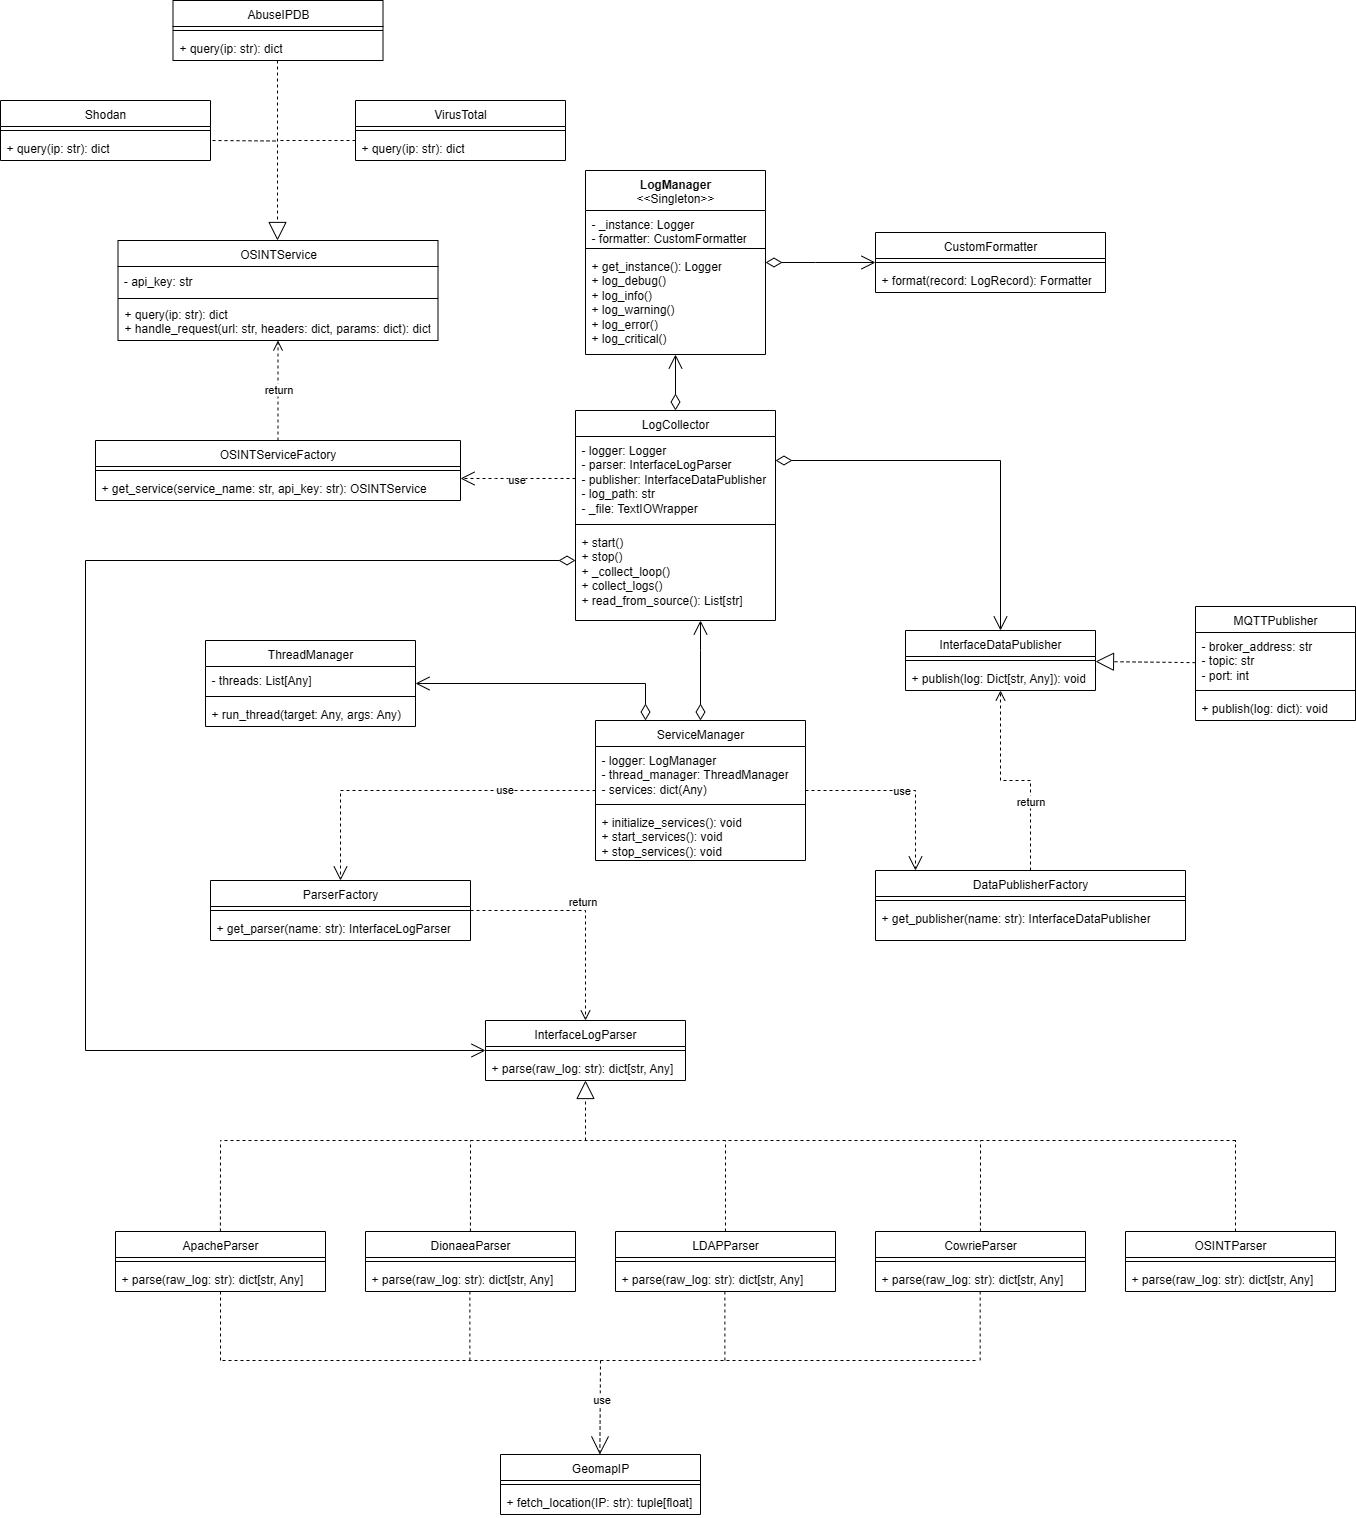
\includegraphics[width=\textwidth]{img/Diagramma-classi.png}
    \caption{Diagramma delle classi del sistema \textit{honeypot}.}
    \label{fig:class-diagram}
    \end{center}
\end{figure}
Per la progettazione del sistema e la realizzazione del relativo diagramma ho applicato diversi \textit{design pattern} studiati durante il corso di Ingegneria del \textit{Software}. 
Un primo esempio è rappresentato dal \textbf{\textit{Factory pattern}}, utilizzato nella classe \textit{ParserFactory}, la quale ha il compito di istanziare i diversi oggetti \textit{parser} a seconda del servizio vulnerabile da analizzare. 
In questo modo la logica di creazione viene centralizzata e resa indipendente dal resto del sistema, favorendo estendibilità e manutenibilità. 
Un ulteriore contributo deriva dall'applicazione dell'\textbf{\textit{Adapter pattern}}, che ha permesso di uniformare i \textit{log} provenienti da sorgenti differenti adattandoli al formato richiesto dal \textit{publisher} \textit{MQTT}; tale approccio consente di integrare componenti con interfacce distinte senza doverne modificare l'implementazione originaria. 
La gestione centralizzata dei \textit{log} è invece garantita dal \textbf{\textit{Singleton pattern}}, applicato alla classe \textit{LogManager}, che deve esistere in un'unica istanza per tutta la durata dell'esecuzione del programma, evitando così conflitti dovuti alla creazione di istanze multiple. 
Per quanto riguarda le operazioni di \textit{parsing}, ho applicato lo \textbf{\textit{Strategy pattern}}, grazie al quale è possibile definire e incapsulare diverse strategie, una per ciascun servizio vulnerabile, e selezionare dinamicamente quella più appropriata durante l'esecuzione. 
L'\textbf{\textit{Observer pattern}} risulta applicato in maniera implicita attraverso l'uso del protocollo \textit{MQTT}: i moduli di monitoraggio pubblicano i \textit{log} su specifici \textit{topic}, ai quali \textit{Telegraf} si iscrive per ricevere in tempo reale gli aggiornamenti. 
Questo meccanismo riflette il principio dell'\textit{Observer}, in cui i cambiamenti nello stato di un soggetto sono propagati automaticamente a tutti gli osservatori registrati.\\\\
Infine, la seguente tabella riassume le versioni realizzate, gli elementi modellati e il tempo dedicato alle attività di modellazione e configurazione del sistema:
\begin{center}
\begin{longtable}{|p{0.25\textwidth}|p{0.10\textwidth}|p{0.25\textwidth}|p{0.05\textwidth}|}
\hline
\multicolumn{1}{|c|}{\textbf{Artefatto}} & 
\multicolumn{1}{c|}{\textbf{Versioni create}} & 
\multicolumn{1}{c|}{\textbf{Elementi modellati}} & 
\multicolumn{1}{c|}{\textbf{Ore dedicate}} \\ 
\hline
\endfirsthead

\multicolumn{4}{c}{{\bfseries \tablename\ \thetable{} -- Continuo della tabella}}\\
\hline
\multicolumn{4}{|c|}{\textbf{Attività di modellazione e configurazione}} \\ \hline
\endhead

\hline \multicolumn{4}{|r|}{{Continua nella prossima pagina...}} \\ \hline
\endfoot

\endlastfoot

Diagramma di flusso sistema & 3 & 8 componenti principali & 12 \\ \hline
Diagramma delle classi \textit{UML} & 4 & 21 classi, 5 \textit{design pattern} & 28 \\ \hline
Configurazione servizi \textit{honeypot} & 4 per servizio & 4 servizi (\textit{Cowrie, Dionaea, Apache, LDAP}) & 40 \\ \hline

\caption{Tabella quantitativa delle attività di modellazione e configurazione.}
\label{tab:modellazione-configurazione}
\end{longtable}
\end{center}